\subsection{An\'alisis de temperatura y tiempos en funci\'on de las discretizaciones}
A continuaci\'on presentamos el an\'alisis y las conclusiones obtenidas de acuerdo a la experimentaci\'on realizada.
Como pudimos intuir en un primer momento, una mayor granularidad en la discretizaci\'on hace escalar r\'apidamente la cantidad de ecuaciones y variables involucradas, con lo que el tiempo de los algoritmos escala r\'apidamente. Como supusimos, ambos algoritmos (Lease, la Eliminaci\'on Gaussiana explotando la estructura banda y la factorizaci\'on LU) utilizados en el an\'alisis,  presentan diferencias de tiempo considerables, sobre todo a partir del \'ultimo caso analizado donde se termina resolviendo un sistema de ecuaciones representado en una matriz de $200 \times 200$
A continuaci\'on se presenta una lista con la granularidad utilizada y el tiempo obtenido para cada algoritmo:


\begin{table}[h]
\begin{tabular}{lll}
Granularidad & Gauss & LU \\
2 & 4.678 & 15.877 \\
1 & 41.381 & 143.102 \\
0.5 & 459.756 & 1784.492 \\
0.1 & 259967.136 & 1058285.72 \\
\end{tabular}
\end{table}



\begin{center}
 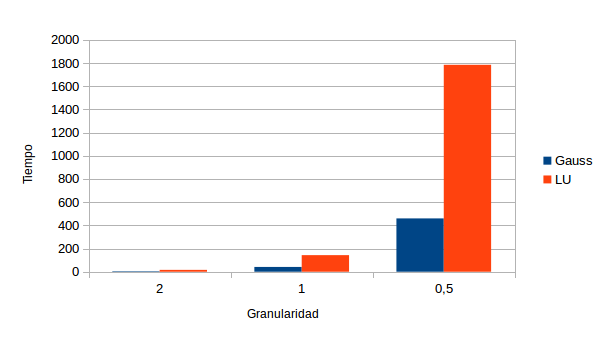
\includegraphics[width=400pt]{imagenes/grafico.png}
\end{center}


En cuanto a la distribuci\'on de calor, partiendo de la base de que un aumento en la granularidad permite una mejor representaci\'on de las sanguijuelas (son circulos), notamos que con este aumento y mejora en la representaci\'on, las temperaturas del punto cr\'itico disminuyen considerablemente. Teniendo en cuenta esta informaci\'on, queda claro como una baja granularidad impacta directamente sobre la precisi\'on de los resultados (a expensas, como vimos con anterioridad, de los tiempos de c\'omputo).

\\
\begin{itemize}
 \item Matriz $20 \times 20$, granularidad 2.\\
  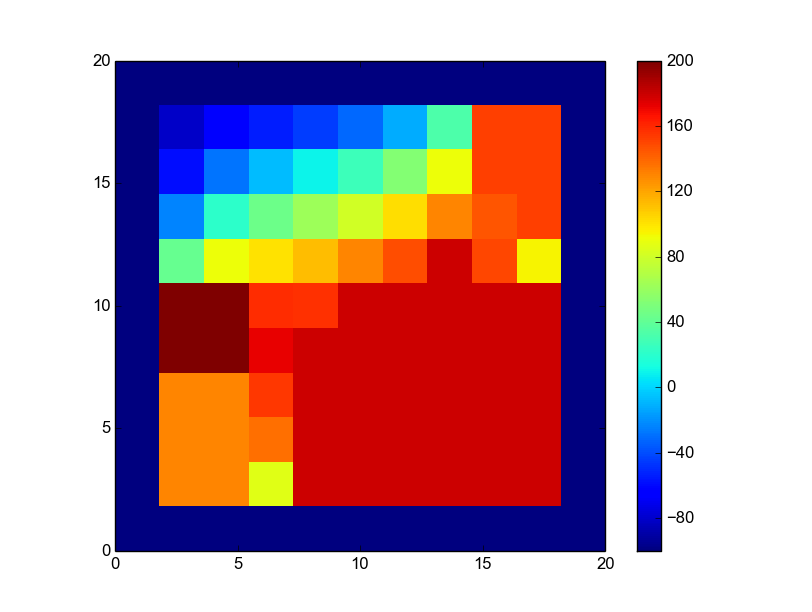
\includegraphics[width=400pt]{imagenes/imagen11.png}

 \item Matriz $20 \times 20$, granularidad 1.\\
  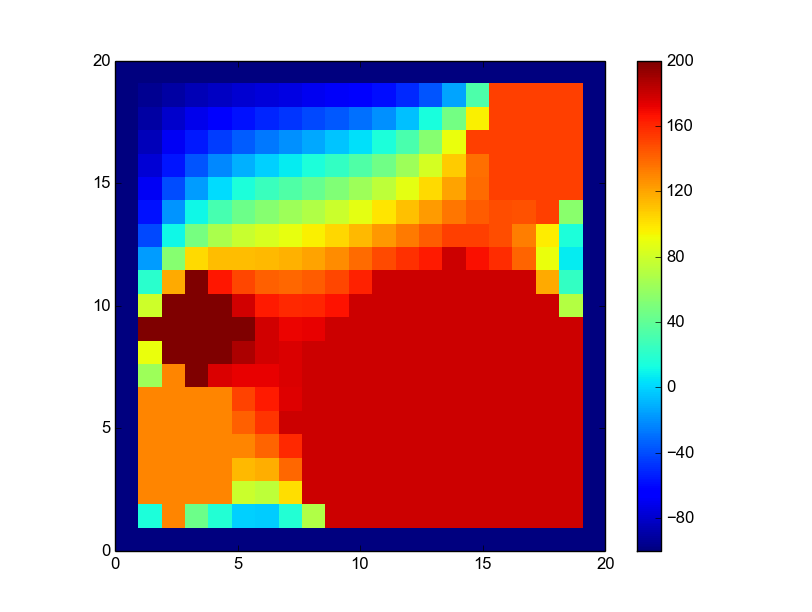
\includegraphics[width=400pt]{imagenes/imagen21.png}

 \item Matriz $20 \times 20$, granularidad 0,5.\\
  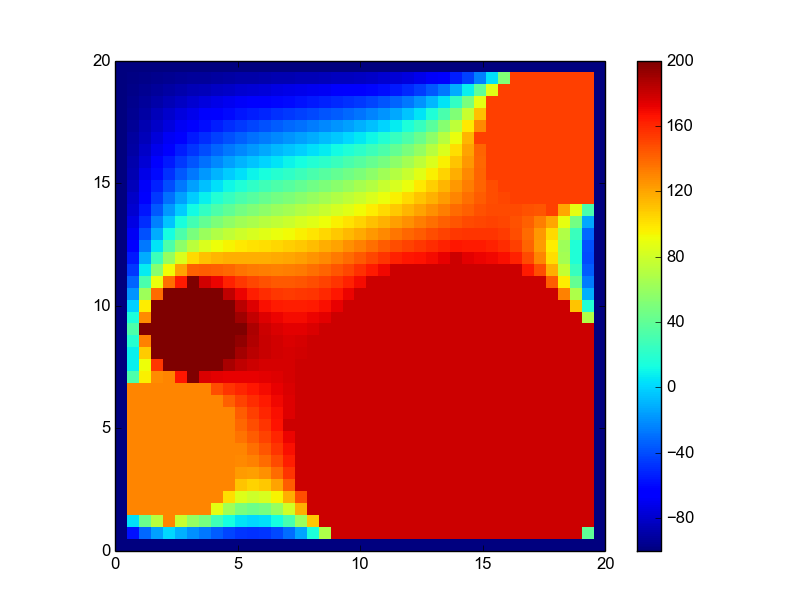
\includegraphics[width=400pt]{imagenes/imagen31.png}
  
   \item Matriz $20 \times 20$, granularidad 0,1.\\
  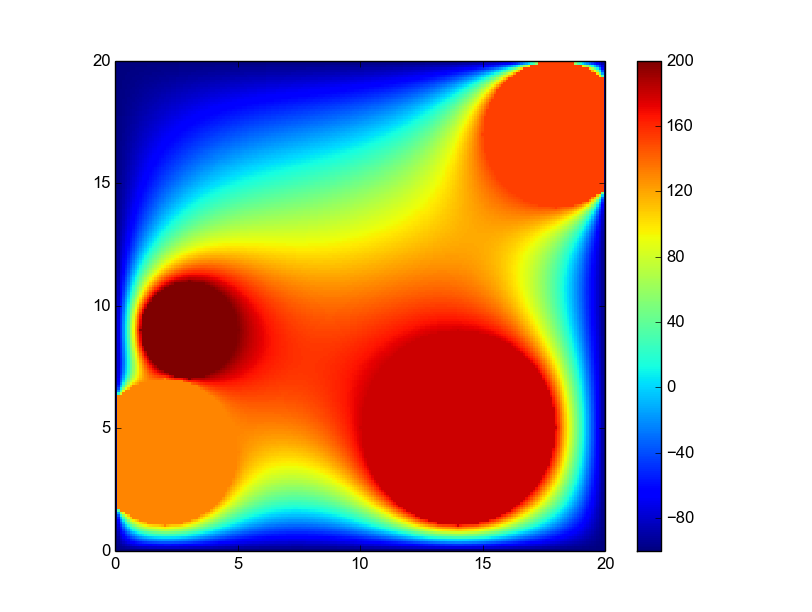
\includegraphics[width=400pt]{imagenes/imagen41.png}
\end{itemize}


Ademas se hicieron test de stress con matrices de $50 \times 50$ generadas de forma aleatoria con una misma semilla y variando la granularidad para analizar la performances de los distintos algoritmos

Algoritmo de salvacion:
\begin{center}
 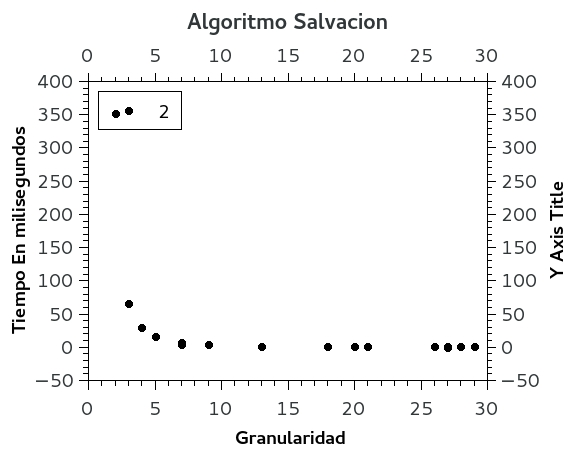
\includegraphics[width=400pt]{graficas/algoritmo salvacion.jpg}
\end{center}

Algoritmo de eliminacion gaussiana:
\begin{center}
 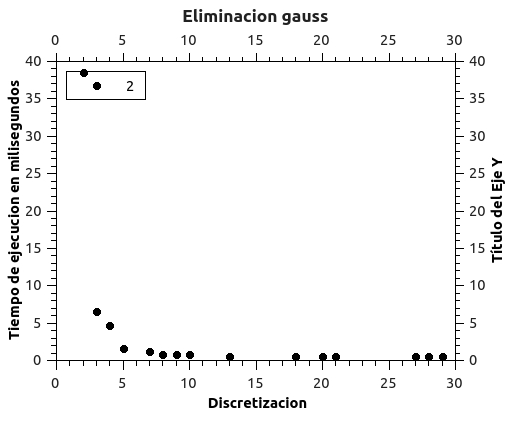
\includegraphics[width=400pt]{graficas/gauss.jpg}
\end{center}

Algoritmo de LU:
\begin{center}
 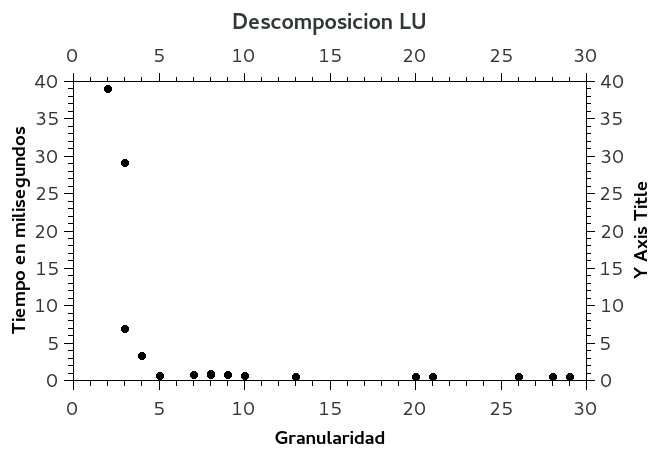
\includegraphics[width=400pt]{graficas/LU.jpg}
\end{center}

\subsection{Optimizaci\'on del c\'omputo para cambios leves del sistema}

As\'i como la particularidad de que el problema se puede plantear mediante el uso de una matriz banda permite ahorrar tiempo de c\'omputo y almacenamiento, otras especificidades del sistema o casos particulares permiten mejorar las estrategias de resoluci\'on. Para casos donde el sistema se modifica levemente, es decir que se produce un cambio en una sola fila de la matriz banda de resoluci\'on, es posible aplicar lo que se conoce como la f\'ormula de Sherman-Morrison. Lo que permite esta f\'ormula es evitar recomputar el algoritmo de eliminaci\'on gaussiana en estos casos, resumiendolo a una peque\~na cantidad de operaciones aritm\'eticas.

Para los casos donde aplica la f\'ormula de Sherman-Morrison, El c\'alculo sobre variaci\'on del sistema se realiza bajo una complejidad computacional de $O(n^2)$ mientras la resoluci\'on a trav\'es de la eliminaci\'on gaussiana cl\'asica es de $O(n^3)$, notando una mejora sustancial usando Sherman-Morrison.

Si bien notamos esta mejora te\'orica y entendemos por qu\'e sucede, no pudimos traducir esta mejora al c\'odigo. Es decir, en los resultados obtenidos no se nota una mejor\'ia respecto al caso base que es la aplicaci\'on de la Eliminaci\'on Gaussiana. Atribuimos esta diferencia entre los resultados te\'oricos y los observados a errores en el c\'odigo y/o en las mediciones ya que no se presentan otros motivos para que los tiempos se mantengan m\'as bajos utilizando Sherman-Morrison.
